\subsection{Training}\label{subsec:training}
Es gibt verschiedene Modelle, die für das Training genutzt werden können.
Die wesentlichen Unterschiede sind:
\begin{itemize}
    \item \textbf{SAEHD (6GB+):} Sparse Auto Encoder HD – geeignet für GPUs mit mindestens 6GB VRAM.
    Einstellbar und für die meisten Benutzer empfohlen.
    \item \textbf{AMP (6GB+):} Neues Modell mit unterschiedlicher Architektur, das versucht, die Form des \texttt{src}-gesichtes beizubehalten.
    Für GPUs mit mindestens 6GB VRAM.
Das AMP-Modell befindet sich noch in der Entwicklung.
    Es wird empfohlen, zunächst mit SAEHD zu arbeiten.
    \item \textbf{Quick96 (2-4GB):} Einfacher Modus für GPUs mit 2-4GB VRAM.
    Feste Parameter: 96x96 Pixel Auflösung, \texttt{whole-face}, Batchgröße 4, DF-UD-Architektur.
    Wird hauptsächlich für schnelle Tests verwendet.
\end{itemize}.
Für das exemplarische Training wurde zu erste ein Testmodell mit \texttt{Quick96} trainiert.
Und anschließend das richtige Modell mit der \texttt{SAEHD}-Architektur erstellt.

Für die Konfiguration der Modelle sind ebenfalls einige Einstellungsmöglichkeiten vorhanden.
Einige davon können nach der Initiierung nicht mehr geändert werden, da diese großen strukturellen Einfluss auf das Modell haben.
Dazu gehören:
\begin{itemize}
    \item Model resolution (Oft abgekürzt mit: ``res'')
    \item Model architecture (``archi'')
    \item Models dimensions (``dims'')
    \item Face type
    \item Morph factor (nur bei AMP training)
\end{itemize}

\subsubsection*{Trainingskonfiguration}
Die Konfiguration von DeepFake-Modell-Trainingsparameter bietet eine Vielzahl von Optionen, um die Qualität und Effizienz des Trainings zu optimieren.
Nachfolgend wird auf die verschiedenen Parameter und deren empfohlene Einstellungen ausführlich eingegangen:

\textbf{Autobackup every N hour (0-24):} Diese Option ermöglicht die automatische Sicherung des Modells in regelmäßigen Abständen.
Ein Wert von 0 deaktiviert diese Funktion.
Die automatische Sicherung ist besonders wichtig, um den Verlust von Trainingsfortschritten zu vermeiden.
Im Falle eines unerwarteten Systemabsturzes oder anderer Probleme kann das Modell von der letzten Sicherung wiederhergestellt werden.
Die Backups bewegen sich je nach \texttt{Resolution} zwischen mehreren Hundert MB und einigen GB.
Ein Modell mit $224$ \texttt{res} war im Test ca. 500MB groß, ein $384$ \texttt{res} schon ca. 2GB.\\

\textbf{Write preview history (y/n):} Diese Einstellung speichert Vorschaubilder während des Trainings in regelmäßigen Abständen.
Wenn aktiviert, wird im Weiteren abgefragt ob die Bilder zufällig oder manuell ausgewählt werden sollen.
Im zweiten Fall wird ein weiteres Fenster geöffnet, in dem die zu speichernden Bilder manuell ausgewählt werden können.
Das Speichern von Vorschaubildern ist nützlich, um den Fortschritt des Trainings zu überwachen und frühzeitig Probleme zu erkennen.
Beispielsweise können Artefakte oder andere unerwünschte Effekte im Trainingsprozess sofort bemerkt und behoben werden.\\

\textbf{Target iteration:} Diese Einstellung bestimmt, nach wie vielen Iterationen das Training beendet wird.\\

\textbf{Flip SRC faces randomly (y/n):} Das zufällige horizontale Spiegeln der \texttt{src}-Gesichter kann hilfreich sein, um alle Winkel im \texttt{dst}-Datensatz abzudecken.
Durch das Spiegeln können mehr Variationen des Gesichts erzeugt werden, was die Generalisierungsfähigkeit des Modells verbessern kann.
Allerdings kann es zu unnatürlichen Ergebnissen führen, da Gesichter nie perfekt symmetrisch sind und spezifische Merkmale von einer Seite zur anderen übertragen werden können.
Die Funktion sollte nur in frühen Phasen des Trainings oder gar nicht aktiviert werden.
Durch das Auswählen guter Ausgangsvideos werden die Vorteile dieser Option überflüssig.\\

\textbf{Flip DST faces randomly (y/n):} Diese Option verbessert die Generalisierung, wenn das zufällige Spiegeln der \texttt{src}-Gesichter deaktiviert ist.
Durch das Spiegeln der \texttt{dst}-Gesichter können ähnliche Vorteile wie bei den \texttt{src}-Gesichtern erzielt werden, insbesondere wenn das Spiegeln der \texttt{src}-Gesichter deaktiviert ist.
Dies kann die Vielfalt der Trainingsdaten erhöhen und das Modell robuster machen.\\

\textbf{Batch\_size:} Die Batch-Größe beeinflusst die Anzahl der Gesichter, die in jeder Iteration verglichen werden.
Eine höhere Batch-Größe liefert bessere Ergebnisse, da mehr Daten pro Iteration verarbeitet werden, benötigt jedoch mehr VRAM und verlängert die Trainingszeit.
Eine niedrige Batch-Größe kann die Trainingsgeschwindigkeit erhöhen, führt jedoch zu weniger genauen Ergebnissen.
Empfohlene Werte liegen zwischen 6 und 12, um ein gutes Gleichgewicht zwischen Trainingszeit und Ergebnisqualität zu erreichen.\\

\textbf{Resolution (64-640):} Die Auflösung des Modells beeinflusst die Detailgenauigkeit der trainierten Gesichter.
Höhere Auflösungen führen zu detaillierteren Gesichtern, erfordern jedoch mehr Rechenleistung und verlängern die Trainingszeit erheblich.
Diese Einstellung kann während des Trainings nicht geändert werden, daher sollte sie sorgfältig gewählt werden.
Eine höhere Auflösung ist vorteilhaft, wenn die Gesichter im endgültigen Video sehr detailliert sein sollen.\\

\textbf{Face type (h/mf/f/wf/head):} Diese Option legt den zu trainierenden Gesichtsbereich fest:
\begin{itemize}
    \item \textbf{HF (Half Face):} Nur der Bereich vom Mund bis zu den Augenbrauen.
    \item \textbf{MHF (Mid Half Face):} Deckt 30\% mehr des Gesichts ab als HF und reduziert das Risiko, dass wichtige Gesichtsteile abgeschnitten werden.
    \item \textbf{FF (Full Face):} Deckt den größten Teil des Gesichts ab, schließt jedoch die Stirn aus.
    \item \textbf{WF (Whole Face):} Deckt das gesamte Gesicht einschließlich der Stirn ab und sorgt so für eine vollständigere Gesichtsabdeckung.
    \item \textbf{HEAD (Head):} Tauscht den gesamten Kopf aus (nicht geeignet ist für Personen mit langen Haaren).
\end{itemize}

\textbf{AE architecture (df/liae - Varianten):} Diese Option ermöglicht die Auswahl zwischen zwei Hauptarchitekturen des SAEHD-Modells: DF und LIAE sowie deren Varianten.
Jede Variante hat spezifische Vor- und Nachteile:
\begin{itemize}
    \item \textbf{DF:} Bietet eine bessere Ähnlichkeit zum Quellgesicht auf Kosten schlechterer Licht- und Farbanpassung.
Diese Architektur erfordert, dass das Quellset besser an die Winkel und Lichtverhältnisse des Zielsets angepasst ist.
    \item \textbf{LIAE:} Bietet eine bessere Anpassung an Licht und Farbe und ist toleranter gegenüber unterschiedlichen Gesichtsproportionen.
Diese Architektur benötigt mehr VRAM und GPU Leistung.
\end{itemize}

\textbf{AutoEncoder dimensions (32-2048):} Bestimmt die allgemeine Fähigkeit des Modells, Gesichter zu lernen.\\
\textbf{Encoder dimensions (16-256):} Beeinflusst die Fähigkeit des Encoders, Gesichter zu lernen.\\
\textbf{Decoder dimensions (16-256):} Beeinflusst die Fähigkeit des Decoders, Gesichter wiederherzustellen.\\
\textbf{Decoder mask dimensions (16-256):} Beeinflusst die Qualität der gelernten Masken.\\

\textbf{Morph factor (0.1-0.5) (Nur bei AMP):} Beeinflusst, wie stark das Modell die vorhergesagten Gesichter an die Quellgesichter anpasst.
Ein höherer Wert kann zu einer höheren Ähnlichkeit führen, jedoch auf Kosten der Realismus des Zielgesichts.
Empfohlener Wert ist 0.5.\\
\textbf{Masked training (y/n) (Nur bei AMP):} Priorisiert das Training der maskierten Bereiche, um sicherzustellen, dass der Fokus des Modells auf den relevanten Teilen des Gesichts liegt.\\
\textbf{Eyes and mouth priority (y/n):} Verbessert die Schärfe und Detailgenauigkeit der Augen und des Mundes, indem diese Bereiche während des Trainings stärker gewichtet werden.\\
\textbf{Uniform yaw distribution of samples (y/n):} Hilft beim Training von Profilgesichtern, indem es das Modell zwingt, gleichmäßig auf alle Gesichtsrichtungen zu trainieren.
Dies kann besonders nützlich sein, wenn das Quellset nicht viele Profilaufnahmen enthält.\\
\textbf{Blur out mask (y/n):} Macht den Bereich außerhalb der Maske weicher, um eine glattere Übergangszone zu schaffen und Artefakte zu reduzieren.\\
\textbf{Place models and optimizer on GPU (y/n):} Verbessert die Leistung, indem alle Berechnungen auf der GPU durchgeführt werden.
Dies erhöht jedoch den VRAM-Verbrauch erheblich.\\
\textbf{Use AdaBelief optimizer? (y/n):} Erhöht die Genauigkeit und Qualität der trainierten Gesichter durch einen besseren Optimierungsalgorithmus, erhöht jedoch den VRAM-Verbrauch.\\
\textbf{Use learning rate dropout (y/n/cpu):} Beschleunigt das Training und reduziert Fluktuation.
Kann auf der CPU ausgeführt werden, um VRAM zu sparen, was jedoch die Trainingszeit verlängert.\\
\textbf{Enable random warp of samples (y/n):} Wird verwendet, um das Modell zu generalisieren, indem es zufällige Verzerrungen auf die Trainingsbilder anwendet.\\
\textbf{Random hue/saturation/light intensity:} Verbessert die Farbstabilität der Quell-Daten während des Trainings, indem zufällige Änderungen von Farbton, Sättigung und Helligkeit angewendet werden.
Empfohlener Wert ist 0.05.\\
\textbf{GAN power (0.0-5.0):} Wird zur Erzielung schärferer und detaillierterer Gesichter verwendet.\\
\textbf{Face style power (0.0-100.0):} Kontrolliert die Stilübertragung des Gesichts, um die Beleuchtung und Farben des Zielgesichts besser anzupassen.\\
\textbf{Background style Power (0.0-100.0):} Kontrolliert die Stilübertragung des Hintergrunds.\\
\textbf{Color transfer for src faceset (none/rct/lct/mkl/idt/sot):} Methoden zur Anpassung der Farben der Quell-Daten an die Ziel-Daten, um Farbabweichungen zu minimieren:
\begin{itemize}
    \item \textbf{None:} Keine Farbanpassung, kann in manchen Fällen bessere Ergebnisse liefern.
    \item \textbf{RCT (Reinhard Color Transfer):} Basierend auf der Reinhard-Farbübertragung.
    \item \textbf{LCT (Linear Color Transfer):} Passt die Farbdarstellung des Zielbildes an die des Quellbildes an.
    \item \textbf{MKL (Monge-Kantorovitch Linear):} Basierend auf der Monge-Kantorovich-Theorie.
    \item \textbf{IDT (Iterative Distribution Transfer):} Iterative Verteilungstransfermethode.
    \item \textbf{SOT (Sliced Optimal Transfer):} Optimale Transfermethode, die Leistungseinbußen während des Trainings und der Zusammenführung verursachen kann.
\end{itemize}
Welche der Farbtransfer-Algorithmen am besten geeignet ist, muss abhängig vom Datensatz ausprobiert werden.
\textbf{Enable gradient clipping (y/n):} Verhindert den Modellkollaps, der durch die Verwendung verschiedener Funktionen verursacht werden kann.\\
\textbf{Enable pretraining mode (y/n):} Wie bereits in früheren Kapiteln beschrieben.
Sehr empfehlenswert für Modelle mit -D Architekturvarianten.\\[0.5cm]

Nach der Konfiguration des Modells und Training, wird überprüft, ob die genügen Hardware (ins besondere RAM und VRAM) verfügbar ist.
Anschließend startet das Training.
\begin{figure}
    \center
    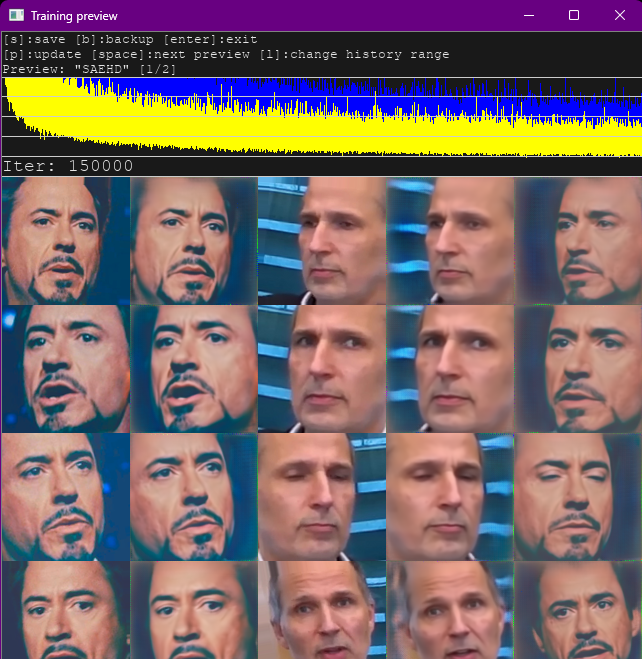
\includegraphics[width=0.7\textwidth]{Bilder/DFL/saehd-train-f}
    \caption{SAEHD Training $128$ \texttt{res}}
    \label{fig:saehd-training}
\end{figure}
Im neu geöffneten Fenster (Abbildung \ref{fig:saehd-training}) sind 5 Spalten zu erkennen.
Diese beinhalten (von links nach rechts):
\begin{enumerate}
    \item Ein Original \texttt{src}-Bild
    \item Die Rekonstruierung des \texttt{src}-Gesichts
    \item Ein Original \texttt{dst}-Bild
    \item Die Rekonstruierung des \texttt{dst}-Gesichts
    \item Das \texttt{src}-Gesicht mit den Ausdrücken des \texttt{dst}-Gesichts
\end{enumerate}
Das Konsolenfenster zeigt nochmals die gewählten Einstellungen, sowie einige anderen Informationen.
\begin{enumerate}
    \item Die aktuelle Zeit
    \item Die aktuelle Iteration
    \item Die Dauer der letzten Iteration
    \item \texttt{src loss value}
    \item \texttt{dst loss value}
\end{enumerate}
\textbf{Loss values} sind Werte die angeben, wie verschieden das rekonstruierte Gesicht vom tatsächlichen Gesicht ist.
Über die Zeit werden diese Werte immer niedriger und gehen gegen Null.
Bei einem unzureichend vorbereiteten Datensatz konvergieren die Werte nicht gegen Null.

\subsubsection*{Trainings Workflow und Ende}
In den Tests hat sich ein Vorgehen herauskristallisiert, dass zu weitestgehend zufriedenstellenden Ergebnissen geführt hat.
Dies bestand aus:
\begin{enumerate}
    \item Pretraining
    \item Training mit \texttt{Uniform yaw distribution of samples} (sonst default)
    \item Training mit \texttt{Eyes and mouth priority}
    \item Default training
    \item Training mit \texttt{GAN Power}
\end{enumerate}
Es lässt sich kein universelles Setup formulieren das über verschiedenes \texttt{src}- und \texttt{dst}-Material hinweg gute Ergebnisse liefert.
Außerdem ist auch bei gut gewählten Einstellungen, das Ausgangsmaterial maßgeblich entscheidend für die Qualität der Deepfakes.

Werden die \texttt{Loss values} nicht mehr kleiner, kann das Training beendet werden.
Außerdem kann in der Preview Ansicht der aktuelle Stand des Modells überprüft werden.
Ein Training kann auch jederzeit wieder fortgesetzt werden, falls die Ergebnisse des exportierten Materials nicht zufriedenstellend sind.\\

Ist ein Modell trainiert, kann dieses als eine \texttt{.dfm}-Datei exportiert werden.
Diese Dateien können in \textbf{DeepFaceLive} importiert und verwendet werden, um Echtzeit Face swapping durchzuführen.
Der Trainingsprozess für ein DeepFaceLive Modell unterscheidet sich in einigen Punkten von dem bisher beschriebenen Prozess und wird in Kapitel \ref{sec:deepfacelive} näher betrachtet.

\subsection{Conversion/Merging}\label{subsec:conversion/merging}
Nach abgeschlossenem Training muss das trainierte Modell noch auf das Zielvideo angewandt werden.
Dafür bietet \gls{dfl} zahlreiche Konfigurationsmöglichkeiten.
Diese sind jedoch von Fall zu Fall verschieden und müssen individuell angepasst werden.
Ein Vergleich einer dieser Konfigurationsmöglichkeiten zeigt Abbildung \ref{fig:merger-comparison}.
\begin{figure}
    \center
    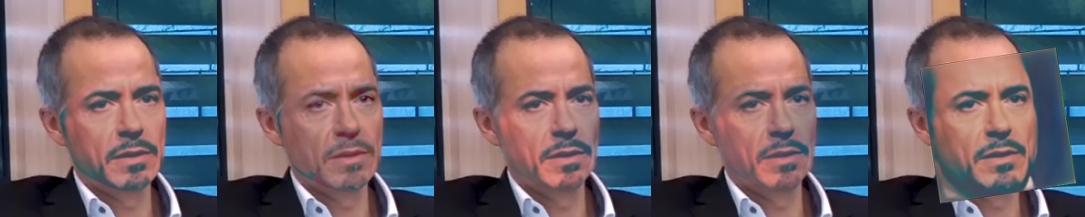
\includegraphics[width=\textwidth]{Bilder/DFL/merger-comparison}
    \caption{Unterschiede: \texttt{overlay}, \texttt{hist-match}, \texttt{seamless}, \texttt{seamless histmatch}}
    \label{fig:merger-comparison}
\end{figure}

Ist das Ergebnis zufriedenstellend, können die neu generierten Bilder wiederrum mit FFmpeg zu einem Video zusammengefügt werden.
\gls{dfl} bietet hierfür wiederrum einen Wrapper.
\begin{lstlisting}[numbers=none,label={lst:merged-to-mp4}]
    8) merged to mp4.bat
\end{lstlisting}